\documentclass[nochap,palatino]{apuntes}

\title{Tratamiento de Señales Visuales}
\author{Guillermo Julián Moreno}
\date{15/16 C1}

% Paquetes adicionales
\usepackage{fancysprefs}
\usepackage{xfrac}
\usepackage{tikztools}
\usetikzlibrary{calc}
% --------------------

\begin{document}
\pagestyle{plain}

\begin{abstract}
Estos apuntes son un pequeño resumen, no exhaustivo, de la asignatura de Tratamiento de Señales Visuales de la EPS UAM. Aquí recogemos todos los conceptos de forma resumida, basándonos en los apuntes proporcionados por los profesores.
\end{abstract}

\maketitle

\section{Operadores puntuales}

Empezamos definiendo las imágenes como aplicaciones $\appl{ψ}{ℝ^2}{I}$, de tal forma que a cada punto $(x,y)$ le asignan un determinado valor de luminosidad. Para imágenes en escala de grises, $I$ será habitualmente $[0,255]$, aunque también podríamos considerar $I = [0,1]$.

Dada una imagen $ψ(x,y)$ de origen, aplicaremos operadores $\appl{T}{ℝ}{ℝ}$ para obtener imágenes de salida $θ(x,y)$. La convención será que la transformación llevará valores $r_k$ a otros $s_k$.

\subsection{Modelado de histograma}

Este tipo de operadores cambian la amplitud de luminosidad de la imagen y se pueden modelar según su efecto en el histograma de la distribución de posibles valores de luminosidad de los píxeles de la imagen. Se puede normalizar para obtener probabilidades entre 0 y 1. Hay tres operaciones principales con operadores puntuales.

\subsubsection{Ajuste de contraste}

El ajuste de contraste pretende expandir ciertas zonas del rango dinámico y comprimir otros para mejorar el contraste de la imagen. Se define como \[
s = T(r) = \begin{cases}
α r & 0 ≤ r < a \\
β(r-a) + s_a & a ≤ r < b \\
γ(r-b) + s_b & b ≤ r < L - 1
\end{cases}
\]

$α,β,γ$ se calculan según los parámetros $a,b,s_a,s_b$ para que $T$ sea continua. En general, la transformación se puede definir como una transformación lineal en tres intervalos: \begin{align*}
[0, a) &\to [0,s_a) \\
[a, b) &\to [s_a, s_b) \\
[b, L - 1] &\to [s_b, L - 1]
\end{align*}

Un posible puede ocurrir debido a la cuantización: al comprimir ciertos rangos, la aplicación puede dejar de ser inyectiva y entonces será imposible recuperar esa información al restaurar el contraste.

\subsubsection{Igualación de histograma}

La igualación de histograma pretende obtener un histograma lo más uniforme posible. La transformación se define como \[ s = T(r) = \sum_{i=0}^r P(I = i) = P(I <= r) \] donde $P(I = i)$ es la probabilidad de que un determinado píxel de la imagen de entrada tenga valor $i$. En otras palabras, se hace una transformación usando como ``tabla de referencia'' la CDF de luminancia.

Se pueden usar otras funciones como tabla siempre y cuando sean monótonas crecientes. Además, también se puede realizar la ecualización adaptativa realizando el proceso de ecualización en porciones de la imagen. Se puede usar ventana deslizante o bien considerar ventanas con solapamiento.

\subsubsection{Especificación de histograma}

La idea es transformar el histograma de una imagen para que se parezca al de otra imagen. Se hace una correspondencia por percentiles. Sea $F$ la CDF del histograma de la imagen a modificar y $G$ la de la imagen especificada. Entonces, se define la transformación $T$ como \[ s = T(r) = \inf \set{i ∈ [0, L-1] \tq G(i) ≥ F(r) }\]

\subsection{Modificación de niveles}

\subsubsection{Recorte y umbralización}

El recorte sirve para eliminar ruido si se sabe que los niveles de la imagen están en un rango $[a,b]$, llevándolos a un rango final $[s_a, s_b]$. La transformación se define como \[ s = T(r) = \begin{cases} s_a & 0 ≤ r < a \\
α(r - a) + s_a & a ≤ r < b \\
s_b & b ≤ r < L - 1
\end{cases} \] con $α = \frac{s_b - s_a}{b - a}$, esto es, el parámetro que hace que $T$ sea continua.

Cuando $a = b = u$, lo que se realiza es una umbralización, lo que nos permite separar objetos según su luminosidad. El umbral $u$ se puede obtener por un algoritmo iterativo. Dado un umbral $u_i$, se define el siguiente umbral como \[ u_{i + 1} = \frac{\avg{A_i} + \avg{B_i}}{2}\], donde $\avg{A_i}, \avg{B_i}$ son los conjuntos de valores por encima y por debajo respectivamente del umbral $u_i$. El proceso se para cuando la diferencia entre umbrales es menor que uno. El primer umbral $u_0$ se suele tomar como la mitad del rango del histograma, esto es, \[ u_0 = \frac{\max ψ - \min ψ}{2} \]

El umbral se puede seleccionar de forma adaptativa considerando una división de ventanas de la imagen.

Una posibilidad es considerar que la distribución del histograma es una normal bimodal. En ese caso, la PDF es \[ p(r) = P_a p_a(r) + P_b p_b(r) \], siendo $P_a, P_b$ coeficientes de ajuste con $P_a + P_b = 1$. El umbral se definiría como \[ u = \frac{μ_a + μ_b}{2} + \frac{σ_b^2}{μ_b - μ_a} \log \frac{P_a}{P_b} \]

\subsubsection{Negativo, seccionado y extracción de bits}

El negativo es simplemente invertir el histograma, con una transformación $s = T(r) = L - 1 - r$.

El seccionado pretende extraer una determinada banda de niveles sobre el resto. Puede ser extracción o resalte. Respectivamente: \[ s = T_E(r) =
\begin{cases}
s_a & r ∉ [a,b] \\
s_b & r ∈ [a,b]
\end{cases} \qquad
s=T_R(r) = \begin{cases}
r & r ∉ [a,b] \\
s_b & r ∈ [a,b]
\end{cases}
\]

La extracción de bits hace lo que uno podría pensar basándose en el nombre. Los valores cuyo bit $n$-ésimo vale $1$ se transforman a $s_b$, y el resto a $s_a$.

\subsubsection{Compresión logarítmica de rango}

La compresión logarítmica de rango viene dada por \[ s = T(r) = (L - 1) \left(\frac{r}{L - 1}\right)^{\frac{1}{γ}} \]

Si $γ > 1$, se trata de una corrección Gamma, y si $γ < 1$, es corrección Gamma inversa (la respuesta de un monitor CRT, por ejemplo).

\subsection{Aspectos operativos}

Al trabajar con valores discretos, tenemos los problemas habituales de redondeos y truncamientos. Pero además tenemos el problema de que hay que hacer $M × N$ cálculos y operaciones, a pesar de que sólo tenemos $L$ posibles valores de enntrada. En la práctica, se puede o bien modificar la VLT (Video Lookup Table, una tabla de $L$ entradas que relaciona un índice en la imagen con su valor real de colores) o montar una Lookup Table (LUT) con todos los posibles valores de entrada y salida y utilizarla para calcular los píxeles de salida de la imagen final sin tener que rehacer los cálculos.

\subsection{Operaciones aritméticas y lógicas}

Se trata de operaciones aritméticas simples sobre dos imágenes. La resta de imágenes permitirá ver errores, eliminar ruido, detectar movimiento o detectar objetos nuevos o desaparecidos. La suma se puede usar para eliminar ruido de media 0 con un promedio de $N$ imágenes, o también para gestionar transparencias

Las operaciones lógicas también se pueden usar, como por ejemplo, con el operador \textit{AND} para obtener regiones de interés de una imagen.

\section{Operadores LSI}

Los operadores lineales e invariantes con el espacio efectúan transformaciones sobre entornos de píxeles dados. Para eso, se usa una ventana deslizante. Este tipo de operaciones tienen un trasfondo de tratamiento de señal, y vamos a verlo formalmente. Dada una transformación $\appl{T}{M_{2a × 2b}}{[0,L]}$\footnote{$M_{i×j}$ es el espacio de matrices de tamaño $i × j$.} que considera entornos rectangulares $A$ de ancho $2a$ y alto $2b$, podemos considerar la respuesta a un impulso unidad $δ$ de tamaño $2a × 2b$, donde $δ[0,0] = 1$ y vale $0$ en el resto de puntos. Esa respuesta viene dada por $h = T(δ)$. La principal ventaja de esto es que al ser $T$ una transformación lineal, podemos definirla únicamente con esa respuesta, ya que cualquier entorno de la imagen origen será una combinación lineales de deltas desplazadas. Así, la transformación completa $\appl{τ}{M_{M×N}}{M_{M×N}}$ de toda la imagen será \[ θ = τ(ψ) = ψ \ast h \], donde $\ast$ es la convolución, que se define para cada píxel de la siguiente forma: \[ θ[n,m] = \sum_{k=-a}^a \sum_{l = -b}^b ψ[n + k, m + l] \cdot h[-k, -l] \]

Por comodidad, consideraremos $w[n,m] = h[-n, -m]$, invirtiendo la respuesta al impulso $h$ y evitándonos que hacer la inversión en cada cálculo.

Al usar la convolución, podemos irnos al dominio frecuencial. Como notación, las letras minúsculas se referirán al dominio espacial y en mayúsculas al dominio frecuencial, pasando de una a otra con la transformada discreta de Fourier. En el dominio frecuencial, la convolución es un producto y por lo tanto \[ Θ = ψ \cdot H \], bastante más fácil de computar.

El problema de este tipo de filtros es que nos comemos los bordes al no tener suficientes píxeles para valorar. Para ello, se puede realizar \textit{padding} aumentando la imagen original. Para rellenar esos píxeles adicionales, se pueden usar valores fijos, hacer una simetría, extender el bore con los mismos valores o hacer una réplica circular con el otro lado de la imagen.

La convolución también tiene la propiedad de separabilidad: si nuestro kernel $w$ se puede expresar como $w = x \otimes y$, siendo $\otimes$ el producto de Kronecker y $x,y$ vectores fila y columna respectivamente, entonces aplicar $w$ es lo mismo que aplicar $x$ y después $y$.

Normalmente, para no modificar el valor medio de la luminosidad de la imagen, ponderaremos $w$ para que la suma de sus elementos sea $1$.

\subsection{Tipos de filtros}

Un filtro simple es la correlación: si ponemos como máscara un objeto, la imagen final destacará las zonas donde ese mismo objeto aparezca. El resto son más complejos y merecen secciones aparte.

\subsubsection{Suavizado}

El suavizado es un filtro paso bajo en frecuencia. Sirve para suavizar o emborronar, y se distingue por tener todos los elementos positivos (realiza una media de los píxeles colindantes).

El promedio puede ser ponderado o no ponderado. Un caso especial del ponderado es el binomial, donde consideramos vectores $B_n$ con los coeficientes binomiales, esto es, con $B_n[i] = {n \choose i}$, y con el filtro $w_n = \frac{1}{2^n} B_n \otimes \trans{B_n}$.

El suavizado también se puede hacer con un filtro de mediana, que suele ser más efectivo filtrando ruido tipo sal y pimienta.

\subsubsection{Realce de contornos}

El realce de contornos se relaciona con la primera y segunda derivada direccionales, versión discreta:
\[ \dpa{f[n]}{n} = f[n+ 1] - f[n]\qquad \pd[2]{f[n]}{n} = f[n+1] + f[n-1] - 2f[n]\]

El estudio de la laplaciana (la suma de las derivadas segundas en las dos direcciones) \[ \nabla^2 ψ = \pd[2]{ψ}{x} + \pd[2]{ψ}{y} \] nos da dos posibles máscaras: la laplaciana $L'$ y la isótropa $I'$, que realzan los bordes:
\[
L' = \begin{pmatrix} 0 & 1 & 0 \\ 1 & -4 & 1 \\ 0 & 1 & 0 \end{pmatrix}
\qquad
I' = \begin{pmatrix} 1 & 1 & 1 \\ 1 & -8 & 1 \\ 1 & 1 & 1 \end{pmatrix}
\]

Normalmente, lo que se quiere hacer es obtener los bordes sin el resto de la imagen, así que las máscaras finales que hacen eso se pueden obtener restando esas máscaras a un único punto obteniendo lo siguiente:
\[
L = \begin{pmatrix} 0 & -1 & 0 \\ -1 & 5 & -1 \\ 0 & -1 & 0 \end{pmatrix}
\qquad
I = \begin{pmatrix} -1 & -1 & -1 \\ -1 & 9 & -1 \\ -1 & -1 & -1 \end{pmatrix}
\]

La Laplaciana nos da la segunda derivada. Para la primera (el gradiente) tenemos varios operadores posibles: Roberts, Prewitt, Sobel y diagonales:
\begin{gather*}
R_1 = \begin{pmatrix} - 1 & 0 \\ 0 & 1 \end{pmatrix} \qquad R_2 = \begin{pmatrix}0 & -1 \\ 1 & 0 \end{pmatrix} \\
P_v = \frac{1}{6} \begin{pmatrix} -1 & -1 & -1 \\ 0 & 0 & 0 \\ 1 & 1 & 1 \end{pmatrix};\,P_h = \trans{P_v}
\qquad
S_v = \frac{1}{8} \begin{pmatrix} -1 & -2 & -1 \\ 0 & 0 & 0 \\ 1 & 2 & 1 \end{pmatrix};\,S_h = \trans{P_v} \\
D^1_1 = \frac{1}{6} \begin{pmatrix} 0 & 1 & 1 \\ -1 & 0 & 1 \\ -1 & -1 & 0 \end{pmatrix};\,D^1_2 = \trans{D^1_1} \qquad
D^2_1 = \frac{1}{8} \begin{pmatrix} 0 & 1 & 2 \\ -1 & 0 & 1 \\ -2 & -1 & 0 \end{pmatrix};\,D^2_2 = \trans{D^2_1}
\end{gather*}

El realce también se puede hacer con filtros diseñados en frecuencia, más concretamente filtros paso alto.

\paragraph{Detección de bordes} La detección de bordes se puede hacer con el realce de contornos. El problema es que los operadores que hemos visto son muy sensibles al ruido, especialmente la laplaciana. Por eso, muchas veces se hace una gaussiana antes (Laplacian of Gaussian)

\subsection{Transformaciones geométricas}

Las transformaciones geométricas mueven los píxeles, normalmente sin cmabiar su valor. Tenemos las transformaciones afines usuales (rotación, escalado, desplazamiento e inclinación) dadas por las respectivas matrices \[
R = \begin{pmatrix} \cos φ & - \sin φ & 0 \\ \sin φ & \cos φ & 0 \end{pmatrix}\quad
E = \begin{pmatrix} ρ_x & 0 & 0 \\ 0 & ρ_y & 0 \end{pmatrix} \quad
D = \begin{pmatrix} 1 & 0 & d_x \\ 0 &  1 & d_y \end{pmatrix} \quad
I = \begin{pmatrix} 1 & -i_x & 0 \\ i_y &  1 & 0 \end{pmatrix} \quad
\]

Para hacer las transformaciones afines, normalmente añadimos un ``1'' al final del vector columna $(x y)$ para poder tener en cuenta los desplazamientos.

Las transformaciones nos permiten corregir distorsiones de la imagen, como la corrección radial o las perspectivas usando proyección geométrica.

\section{Operadores morfológicos}


Los operadores morfológicos implican un tipo de selección distinto al que hemos visto en los LSI. Consideramos dos operadores, supremo ($\vee$) e ínfimo ($\wedge$) y el punto $δ_L(n)$ que vale $0$ cuando $n = 0$ y $- ∞$ en otro caso. Así, una señal cualquiera $x$ se puede representar como \[ x[n] = \bigvee_{k=-∞}^∞ x[k] + δ_L[n-k]\]

\subsection{Dilatación y erosión}

Con el supremo y el ínfimo podemos definir dos operaciones similares a la convolución: la dilatación ($\oplus$) y la erosión ($\ominus$): dado un elemento estructurante $b$, definimos ambos operadores de la siguiente forma para cada punto $y[n]$: \begin{align*}
y[n] = x[n] \oplus b &= \bigvee_{k=-∞}^∞ (x[k] + b[n-k]) \\
y[n] = x[n] \ominus b &= \bigwedge_{k=-∞}^∞ (x[k] + b[n-k])
\end{align*}

\begin{figure}[hbtp]
\centering
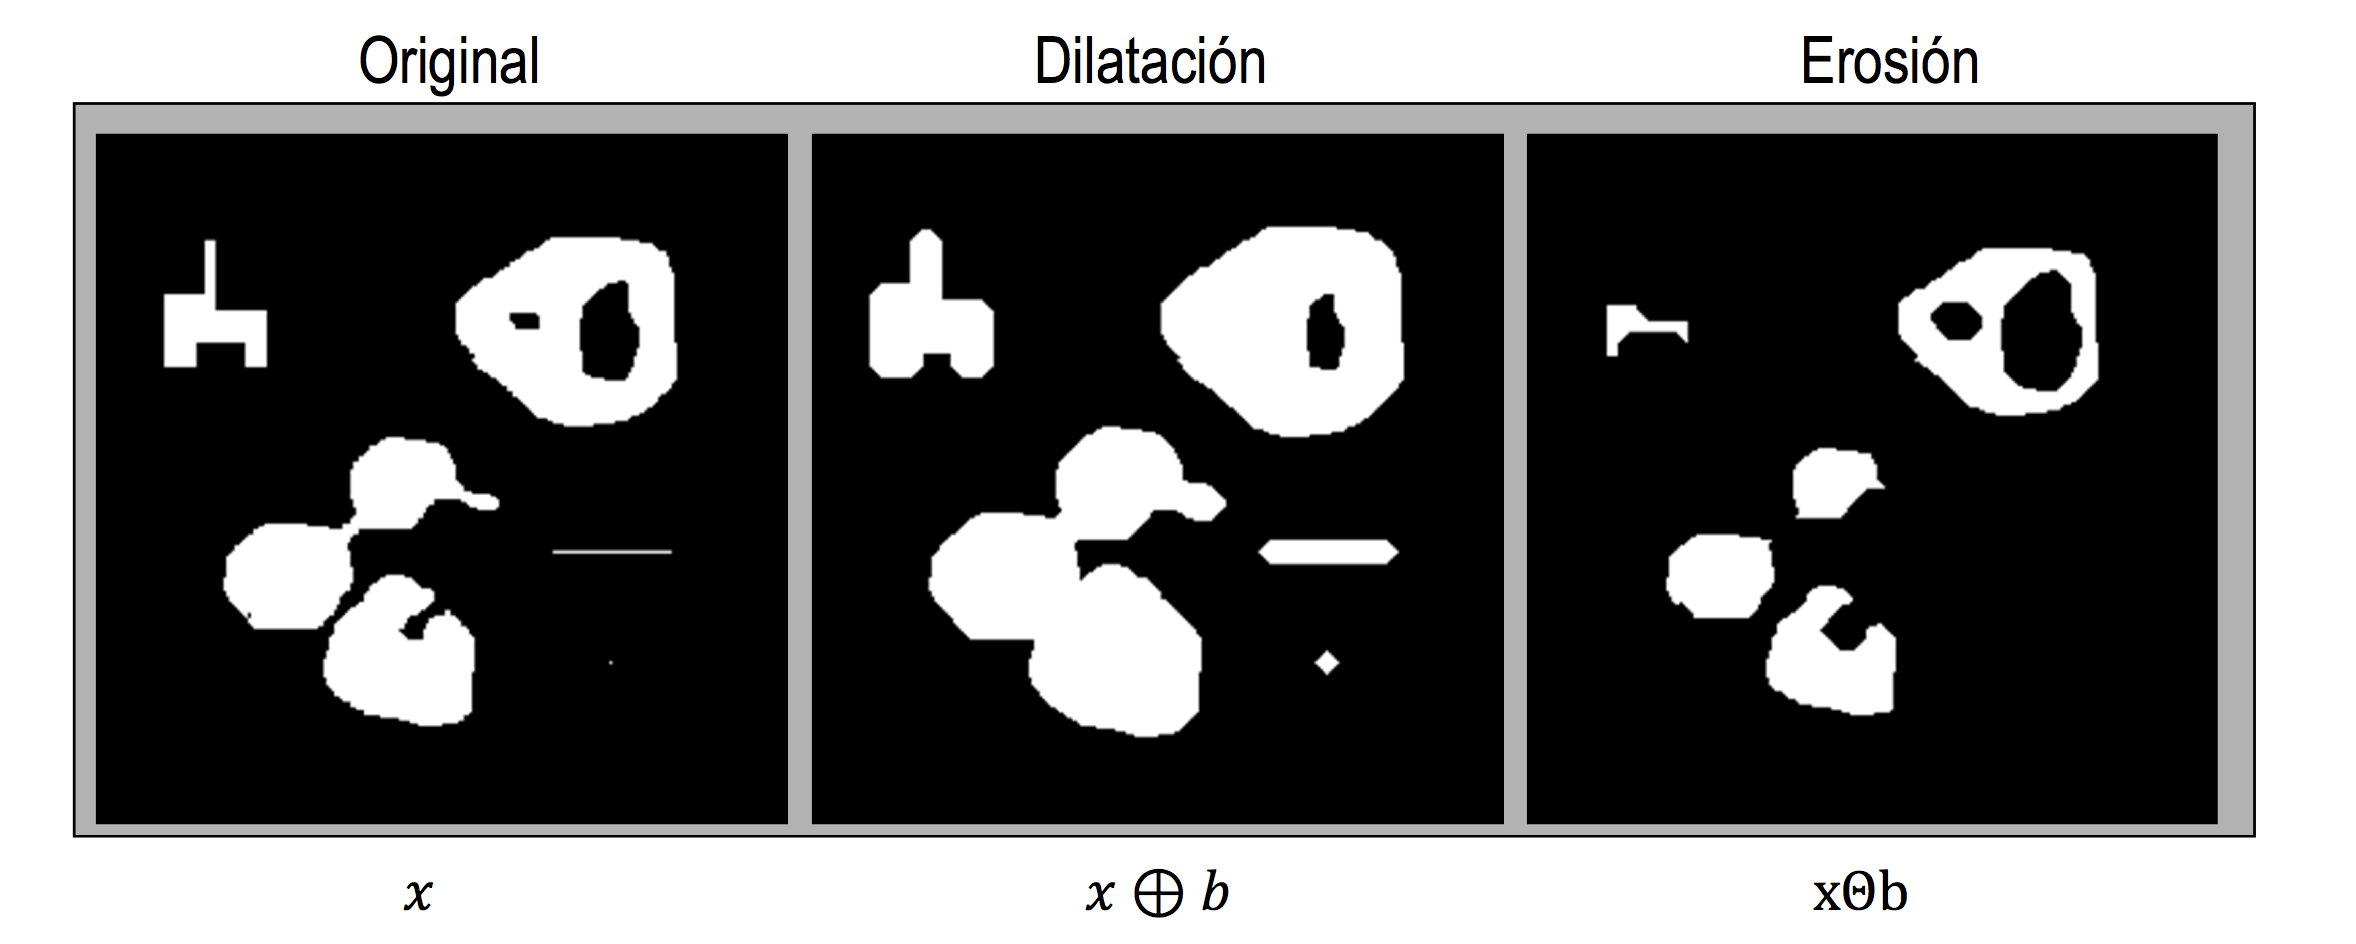
\includegraphics[width=1\textwidth]{img/DilatacionErosion.png}
\caption{Efecto de los operadores dilatación y erosión}
\label{fig:DilatacionErosion}
\end{figure}

En la práctica, la dilatación asigna a un píxel el máximo de todos los píxeles de su entorno que coinciden con los ceros del elemento estructurante invertido. Análogamente, la erosión hace lo mismo pero poniendo el mínimo. El efecto de ambos operadores se puede ver en la \fref{fig:DilatacionErosion}.

La dilatación y la erosión son distributivas con respecto al ínfimo y al supremo:
\begin{align*}
(x \vee y) \oplus b &= (x\oplus b) \vee (y \oplus b) \\
(x \wedge y) \ominus b &= (x\ominus b) \wedge (y \ominus b)
\end{align*}

La composición funciona con la dilatación, pero no del todo bien con la erosión:
\begin{align*}
x \oplus a \oplus b &= x \oplus (a \oplus b) \\
x \ominus a \ominus b &= x \ominus (a \oplus b)
\end{align*}

Si el elemento estructurante incluye el origen, la dilatación es extensiva (los píxeles de salida tienen valor mayor o igual que la entrada) y la erosión antiextensiva (los píxeles de salida tienen valor menor o igual que la entrada).

La dilatación puede reparar objetos, cerrando bordes y quitando imperfecciones (mordidas). La erosión también puede quitar imperfecciones (salidas) y además separar objetos. Ambos operadores pueden ayudar a simplificar imágenes.

\subsubsection{Gradientes morfológicos}

Podemos sacar gradientes por dilatación ($x \oplus b - x$), por erosión ($x - x \ominus b$) o morfológicos ($x\oplus b - x \ominus b$). Si usamos imágenes binarias, deberíamos usar la operación \textit{XOR}.

\subsection{Apertura y cierre}

\begin{figure}[hbtp]
\centering
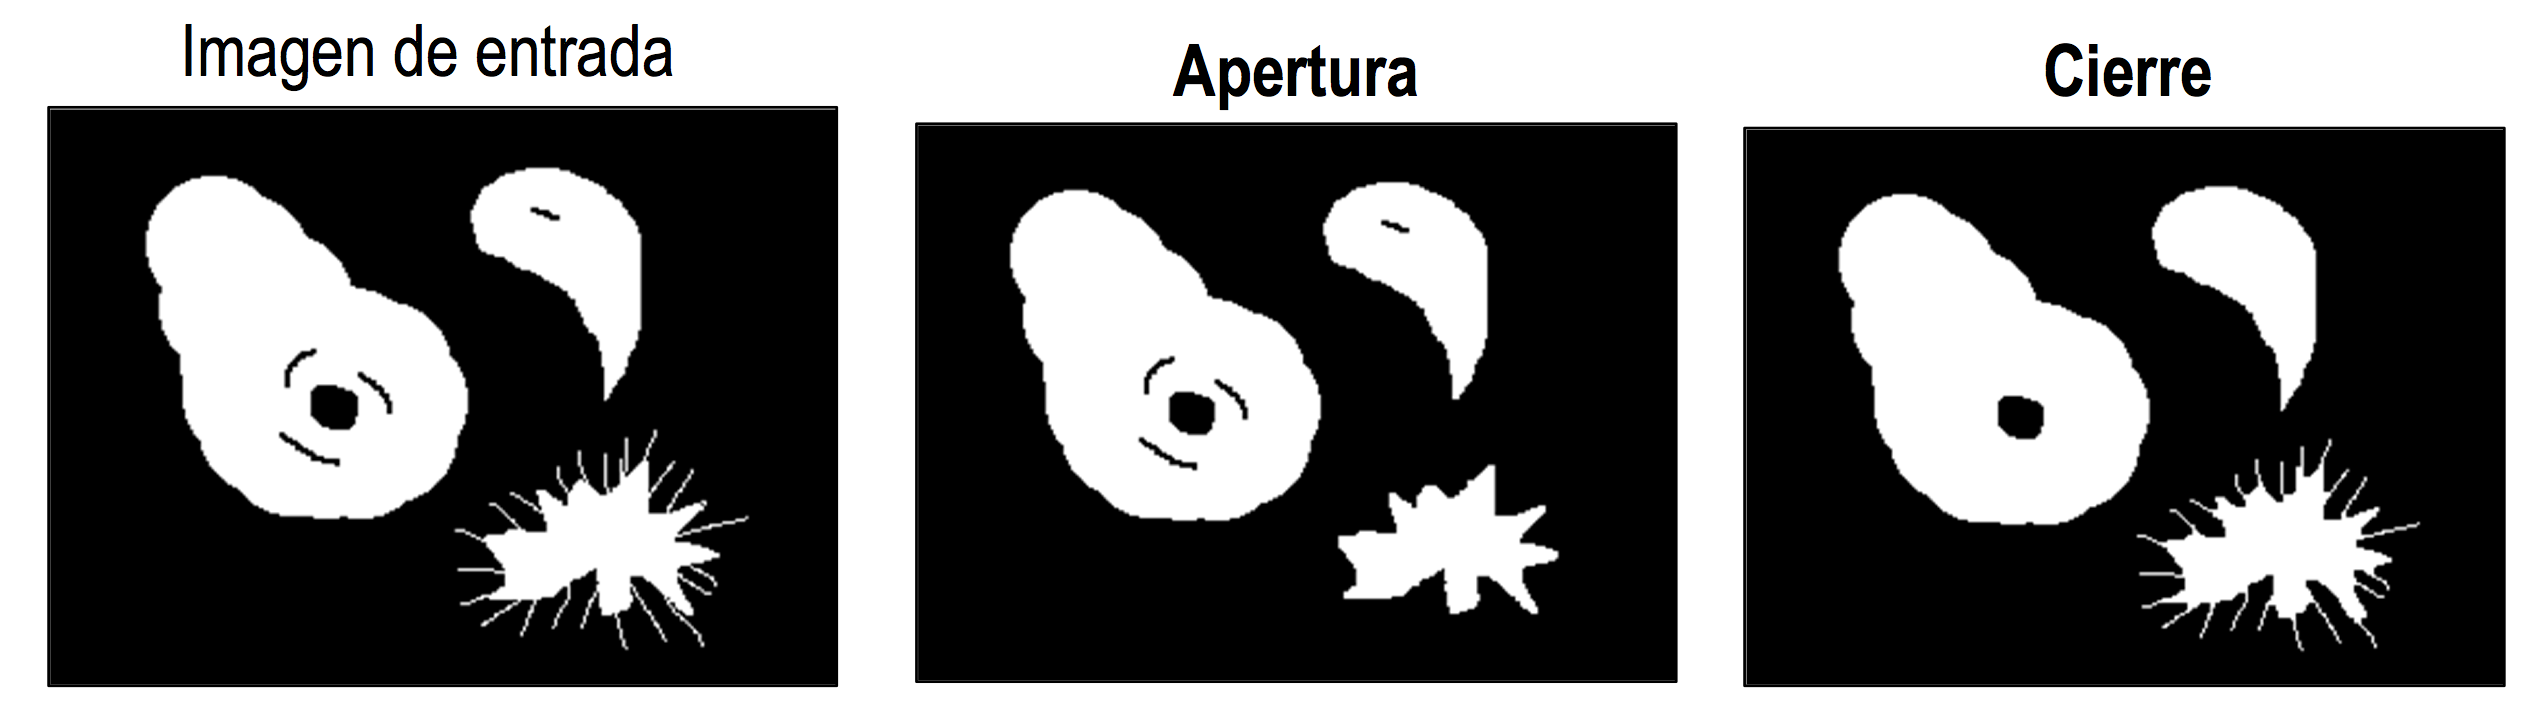
\includegraphics[width=\textwidth]{img/AperturaCierre.png}
\caption{Efecto de los operadores apertura y cierre.}
\label{fig:AperturaCierre}
\end{figure}

Podemos componer los dos operadores básicos para obtener la apertura $γ_b$ y el cierre $φ_b$: \begin{align*}
γ_b &= (x \ominus b) \oplus b \\
φ_b &= (x \oplus b) \ominus b
\end{align*}

El efecto de estos operadores se puede ver en la \fref{fig:AperturaCierre}. La apertura ``abre'' los huecos negros y el cierre ``cierra'' esos mismos agujeros. La apertura es antiextensiva y el cierre extensivo, independientemente de $b$. Además, son idempotentes: sucesivas aplicaciones dan el mismo resultado ($γ(γ(x)) = γ(x)$).

Estos operadores se pueden usar para eliminar objetos de acuerdo a su nivel de gris y de su estructura.

\subsubsection{Detección de objetos}

Se pueden buscar elementos que aparecen como máximos relativos con $x - γ(x)$  (top-hat) y mínimos relativos como $φ(x) - x$ (dual top-hat).

\subsubsection{Granulometría}

\begin{figure}[hbtp]
\centering
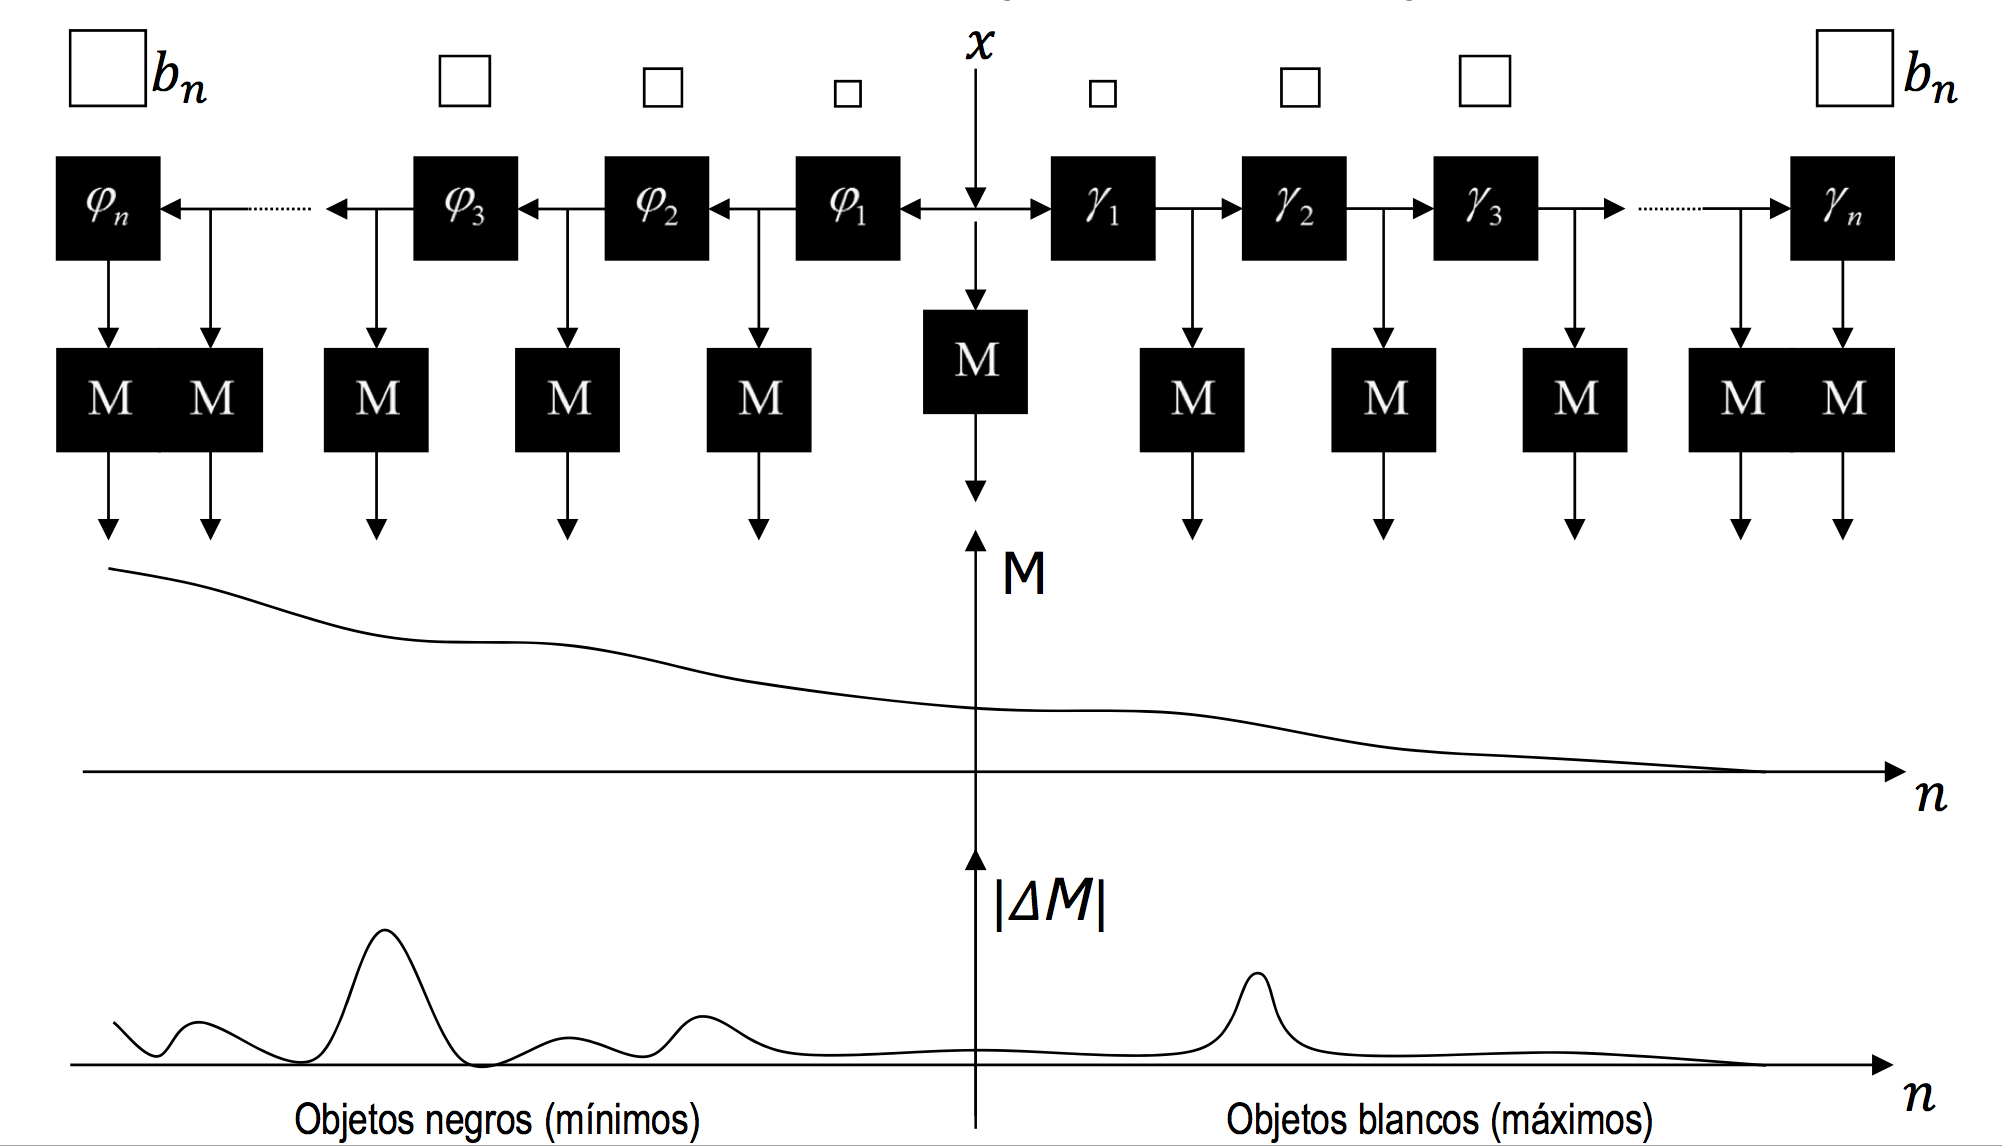
\includegraphics[width=0.9\textwidth]{img/Granulometria.png}
\caption{Granulometría: aplicación sucesiva de aperturas y cierres para detectar cambios en el área.}
\label{fig:Granulometria}
\end{figure}

Aplicando sucesivos bancos de aperturas y cierres (\fref{fig:Granulometria}) con elementos estructurantes crecientes podemos llegar a detectar el tamaño de los objetos.

\subsubsection{Filtrado por reconstrucción}

\begin{figure}[hbtp]
\centering
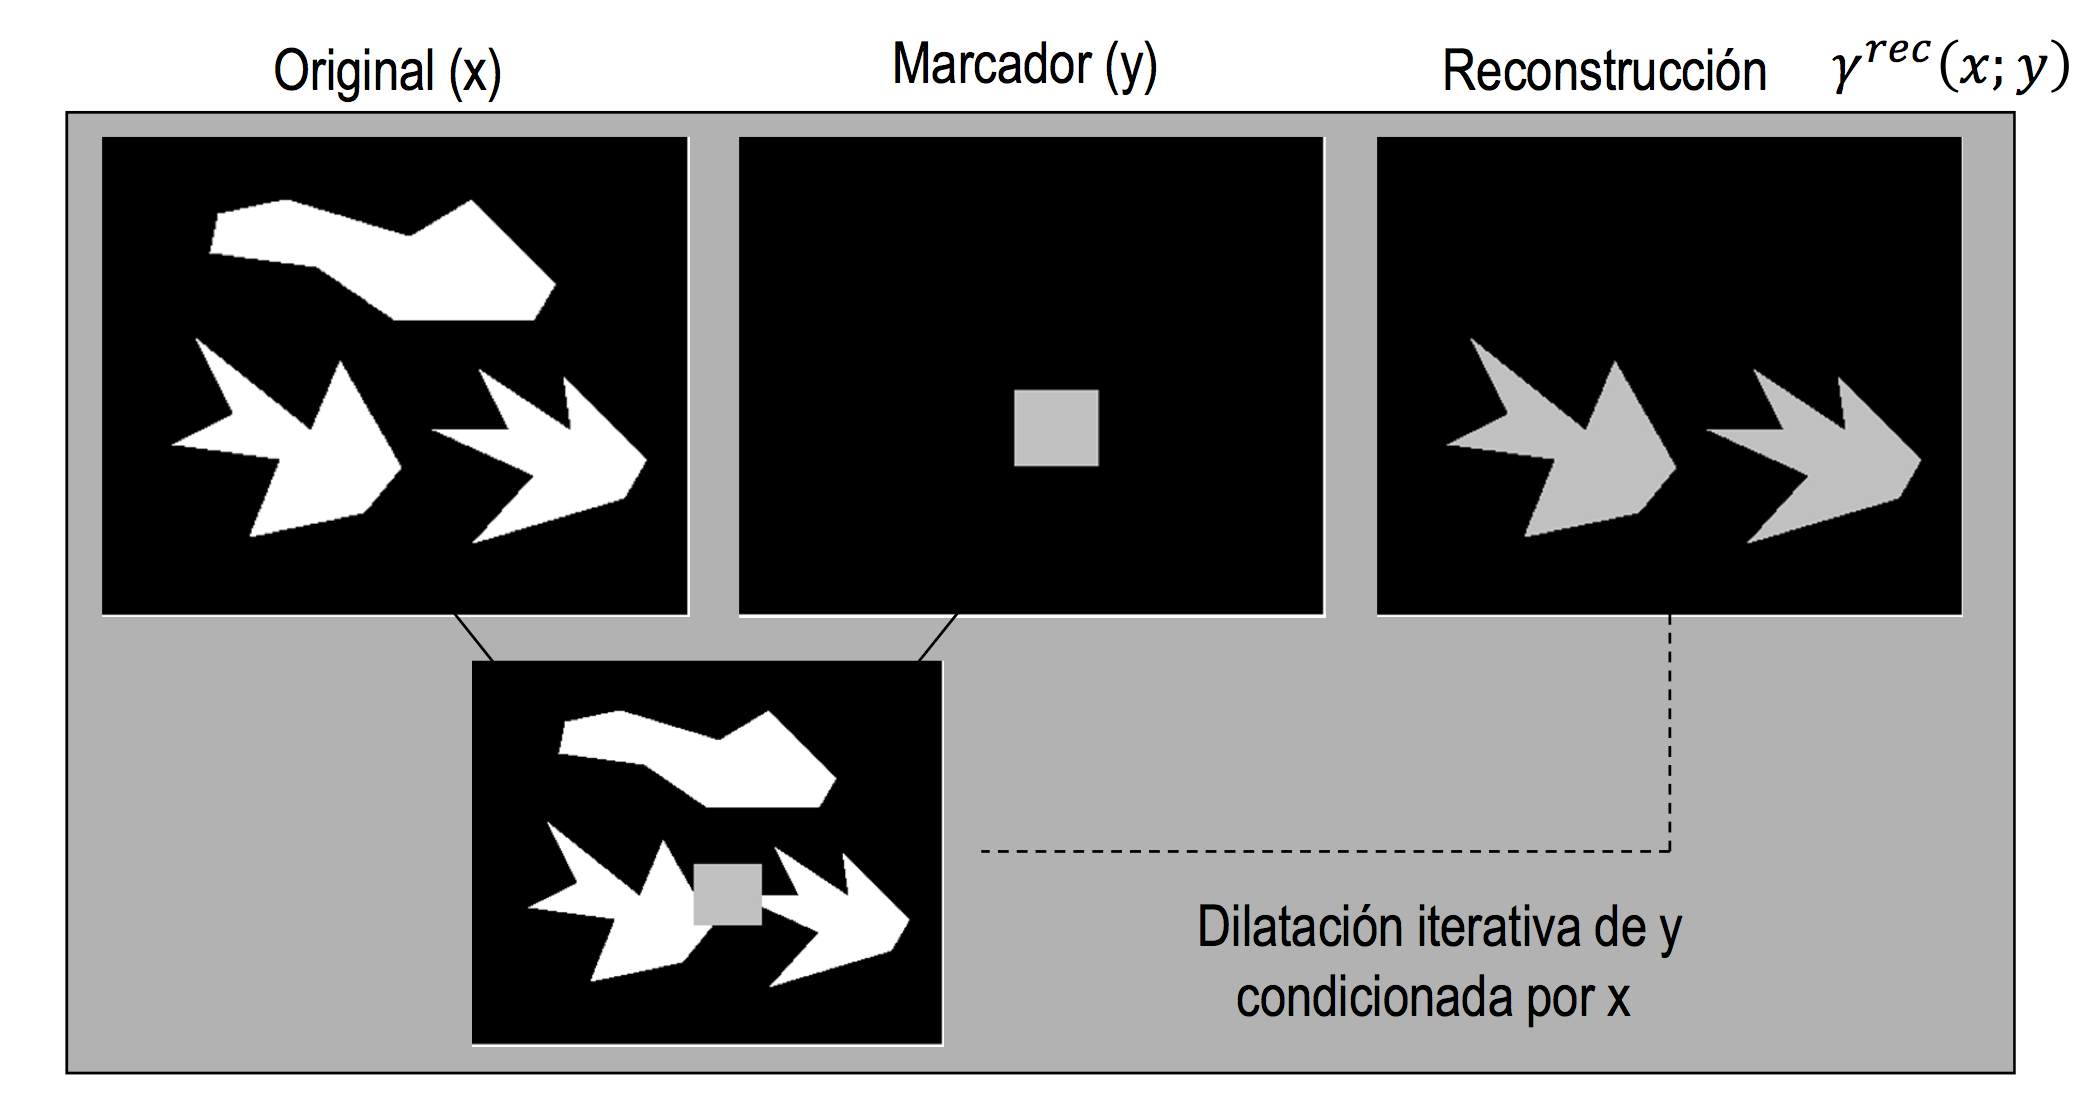
\includegraphics[width=0.9\textwidth]{img/AperturaReconstruccion.png}
\caption{Resultados de la apertura por reconstrucción.}
\label{fig:AperturaReconstruccion}
\end{figure}

Se usan para hacer simplificaciones preservando contornos. Se coge la imagen de entrada $x$, un marcador $y$ y un elemento estructurante que definirá la conectividad de los elementos que mantiene. Se define entonces la apertura y cierre por reconstrucción como un proceso iterativo\begin{align*}
γ^r_i &= (γ^r_{i-1} \otimes b) \wedge x \\
φ^r_i &= (φ^r_{i-1} \ominus b) \vee x
\end{align*} con $γ^r_0 = φ^r_0 = y$. Las operaciones completas se hará con $i \to ∞$, pero por comodidad denotaremos los operadores como $γ^r \equiv γ^r_{∞}$ y $φ^r \equiv φ^r_{∞}$

Tanto la apertura como cierre por reconstrucción tienen las mismas propiedades de extensividad e idempotencia que sus versiones sin reconstrucción.

Normalmente, para el marcador se usarán versiones modificadas de la imagen de entrada, de tal forma que podremos emular la dilatación y erosión sin perder bordes. La apertura mediante reconstrucción de la erosión eliminará ruido más claro que el resto de la imagen, por ejemplo.

También se puede usar este tipo de filtrado para rellenar agujeros, usando un marcador que sea igual a toda la imagen y un cierre por reconstrucción. Un top-hat con la apertura por reconstrucción ($x - γ^r (x;y)$) nos quitará objetos parcialmente visibles si usamos un marcador que sea 1 únicamente en los bordes.

La apertura por reconstrucción de la erosión facilitará el suavizado sin perder los contornos, y el cierre mediante reconstrucción de la dilatación nos permitirá eliminar ruido o elementos pequeños más oscuros sin perder los contornos originales.

\section{Extracción de características}

En este tema trataremos de extraer patrones y características de las imágenes. Una cosa que tendremos que tener en cuenta es la escala de lo que estamos detectando. Esto será lo que se llama el análisis multiescala.

\subsection{Primeras aproximaciones: quad-tree y pirámides}

\begin{figure}
\centering
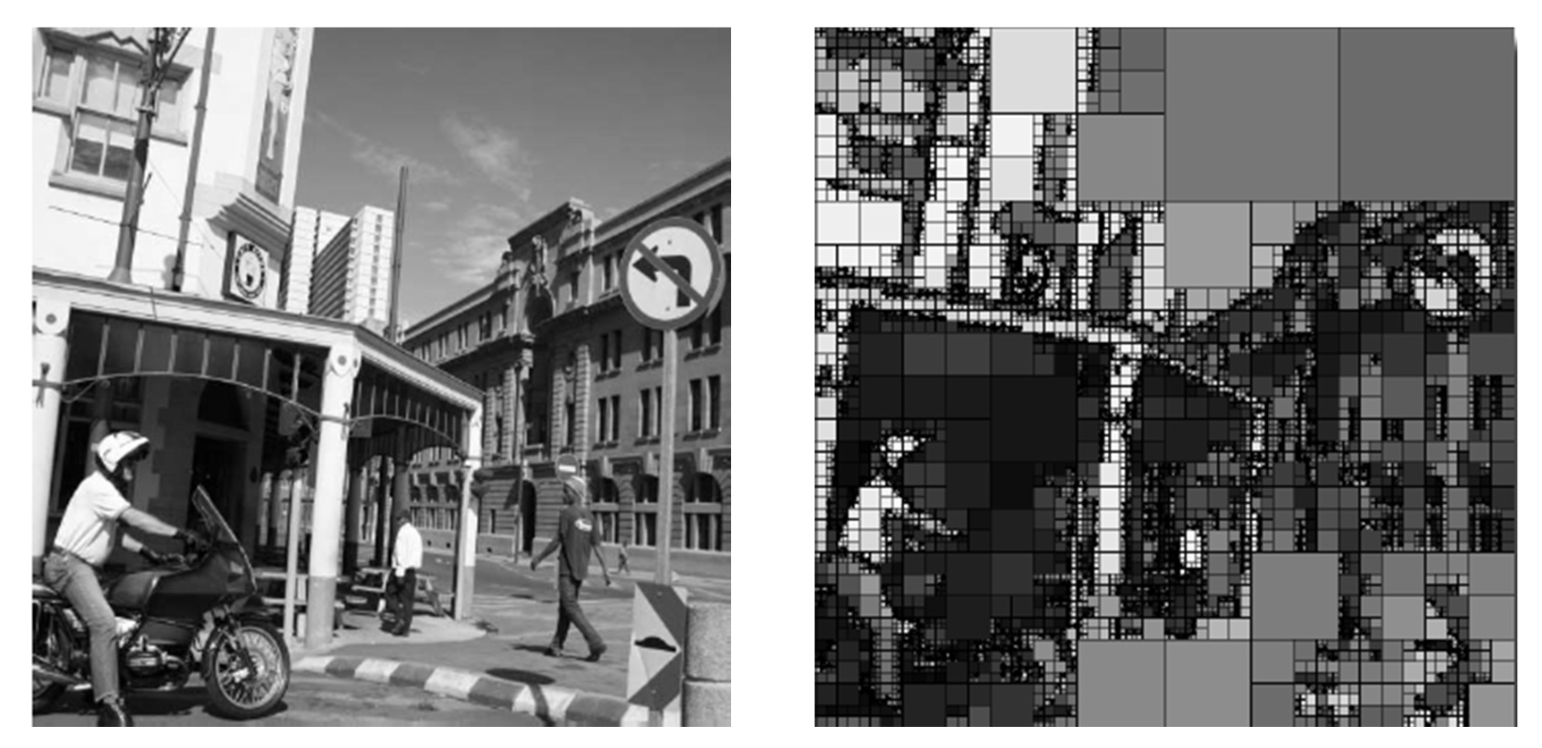
\includegraphics[width=0.8\textwidth]{img/QuadTree.png}
\caption{Representación en quad-tree de una imagen usando criterios de homogeneidad.}
\label{fig:QuadTree}
\end{figure}

Una primera aproximación es la representación en quad-tree (\fref{fig:QuadTree}): seleccionamos un criterio de homogeneidad, un umbral de decisión y un tamaño mínimo de región; y vamos subdividiendo hasta llegar al tamaño mínimo construyendo un árbol por el camino. Salvo esas últimas regiones, el resto cumplen los criterios de homogeneidad.

La segunda aproximación es el uso de repreentaciones piramidales, donde vamos suavizando y diezmando la imagen original para reducir su tamaño. No es un esquema muy formal pero es rápido y computacionalmente barato.

Una ventaja de usar las pirámides es que podemos mandar una imagen en distintas resoluciones sin tener que enviar todos los datos: podemos enviar la imagen original y las diferencias entre niveles, que nos ocuparán menos píxeles.

Podemos usar pirámides paso bajo, donde convolucionamos con un kernel y después reducimos el tamaño a la mitad. El kernel tiene que ser positivo, simetrico, monomodal, de área unidad. Para $N=3$, sólo el dado por $c[n] = \set{\frac{1}{4}, \frac{1}{2}, \frac{1}{4}}$ lo cumple. Para $N=5$, son de la forma \[ c[n] = \set{\frac{1 - 2a}{4}, \frac{1}{4}, \frac{a}, \frac{1}{4}, \frac{1 - 2a}{4}} \]

El siguiente paso es usar las pirámides paso-banda (DoLP, \textit{difference of low-pass pyramids}) en general o, en el caso que más nos interesará, la pirámide laplaciana o DoG \textit{Difference of Gaussians} cuando la pirámide paso-bajo sea Gaussiana (la principal ventaja de usar kernels gaussianos es que minimizamos la aparición de estructuras por \textit{aliasing}). La idea de la pirámide laplaciana es que cada nivel es una aproximación al LoG de la imagen a esa escala.

\subsection{Espacio escala}

En el espacio escala, en lugar de reducir el tamaño de la imagen, lo que haremos será suavizar, y además podremos tomar la variable de suavizado continua. Veremos que usando el kernel gaussiano, tendremos una aproximación perfecta de la LoG. También veremos que es invariante a traslaciones. Por último, el espacio escala no introduce artefactos, estructuras que no existiesen en la imagen.

\begin{defn}[Representación\IS espacio escala] Dada una señal escalar de dimensión $N$ $\appl{ψ}{ℝ^N}{ℝ}$, su representación espacio escala es una aplicación $\appl{L}{ℝ^N × ℝ^+}{ℝ}$ dada por \begin{align*}
L(\vx, 0) &= ψ(\vx) \\
L(\vx, t) &= g(\vx, t) \ast ψ(\vx)
\end{align*} donde $g(\vx, t)$ es la gaussiana dada por \[ g(\vx, t) = \frac{1}{2πt}e^{-\frac{\norm{\vx}}{2t}}\]
\end{defn}

El kernel gaussiano es el único que hace que se cumpla, entre otras cosas, la siguiente ecuación: dados $t_2 > t_1$ entonces \( L(\vx, t_2) = g(\vx, t_2 - t_1) \ast L(\vx, t_1) \label{eq:ScaleSpaceGroup} \) ya que se cumple que \[ g(\vx, σ_1^2) \ast g(\vx, σ_2^2) = g(\vx, σ_1^2 + σ_2^2) \]

El tamaño de la gaussiana que se aplica determina el tamaño de muestreo: un tamaño más pequeño nos dará más precisión en la escala pero costará más calcular.

Otra propiedad útil del espacio escala es que, dadas dos imágenes concretas $I_1, I_2$ y dos filtros gausianos $G_1$, $G_2$ con desviaciones típicas $σ_1, σ_2$ respectivamente, entonces las imágenes $L\ast(G_1 \ast I_1)$ (la laplaciana de la gaussiana) se parece más a $G_1 \ast I_1 - G_2 \ast I_2$ cuanto más se parezcan $I_2$ e $I_1$ y más se parezcan las desviaciones típicas $σ_1,σ_2$.

Más concretamente, y con algo un poco más precisión porque lo de antes es lo menos matemático que he visto en años, si tenemos una imagen $I$ y un kernel gaussiano $G_1$; entonces $L\ast(G_1 \ast I) = (G_1 \ast I) - (G_1 \ast (G_1 \ast I))$ o, en otras palabras, la laplaciana de la gaussiana es igual (salvo un factor de escala) a la diferencia entre las imágenes resultantes de aplicar una y dos veces el kernel $G_1$ a la imagen $I$.

Este hecho nos permitirá obtener la representación en espacio escala de la imagen aplicando iterativamente convoluciones con un kernel fijo, mucho más barato computacionalmente que usando kernels cada vez más grande.

Un hecho importante del espacio escala cumple la ecuación del calor, dada por \[ ∂_t L = \frac{\nabla^2 L}{2} = \frac{1}{2} \sum_{i=1}^N \pd[2]{L}{x_i}\]

Esta propiedad permite inferir que esta representación no realza máximos ni mínimos, y además nos da una pseudodemostración de por qué la LoG y la DoG son equivalentes:
\[ \nabla^2 L(\vx,t) \simeq L(\vx,t + Δt) - L(\vx, t - Δt) \]

También podremos derivar haciendo una ligera perversión matemática: \[ ∂_{x^my^n} L(\vx, t) = ∂_{x^my^n} \left(g(\vx,t) * ψ(\vx)\right) = \left(∂_{x^my^n} g(\vx, t)\right) * ψ(\vx) \], cuya principal ventaja es que las propiedades del espacio escala se trasladan a sus derivadas, por ser la derivada de la gaussiana también una gaussiana.

Este hecho nos permitirá hacer detección inicial de características básicas (blobs), pudiendo detectar también en qué escala se producen. Hay tres métodos para esto: los basados en la LoG, en la DoG, y en el determinante del Hessiano (DoH).

\subsubsection{LoG - Laplacian of Gaussian}

Podemos considerar la laplaciana en las direcciones espaciales. Simplificando y tomando $L_{xx} = \pd[2]{L}{x}$, diremos que  \[ \nabla^2 L = L_{xx} + L_{yy}\], que tomará grandes valores negativos y positivos para bloques claros y oscuros de anchura $2 \sqrt{t}$. La respuesta, eso sí, dependerá de la escala y decrece según esta aumenta, así que para evitarlo se normaliza con respecto de la escala,  de tal forma que nos quedará \[ \nabla^2_{\text{norm}} = t(L_{xx} + L_{yy}) \]

En ese operador buscaremos máximos y mínimos locales, que nos darán puntos y escalas de las regiones más claras y oscuras, respectivamente, del espacio escala.

\subsubsection{DoG - Difference of Gaussians}

En este caso simplemente hacemos lo mismo que en el LoG, pero implementando el operador laplaciano como \[ \nabla^2_{\text{norm}} L(\vx, t) \simeq \frac{t}{Δt} \left(L(\vx, t + Δt) - L(\vx, t - Δt)\right)\] y buscando máximos y mínimos locales.

\subsubsection{DoH - Determinant of Hessian}

El Hessiano de la imagen ψ será una amtriz cuadrada con las segundas derivadas parciales de la función. Su cálculo en puntos críticos (gradiente nulo) y el posterior estudio de los autovalores nos dirá el tipo de punto: autovalores positivos implican mínimo, negativos implican máximo, y mixtos punto de silla.

Al ser el determinante el producto de autovalores, sólo tendremos que calcular eso: si es positivo, es máximo o mínimo, y si es negativo estamos en un punto de silla. Así, sólo tenemos que buscar los máximos locales en el determinante normalizado: \[ \det H_{\text{norm}}L(\vx, t) = t^2 (L_{xx} L_{yy} - L^2_{xy})\]

\begin{figure}[hbtp]
\centering
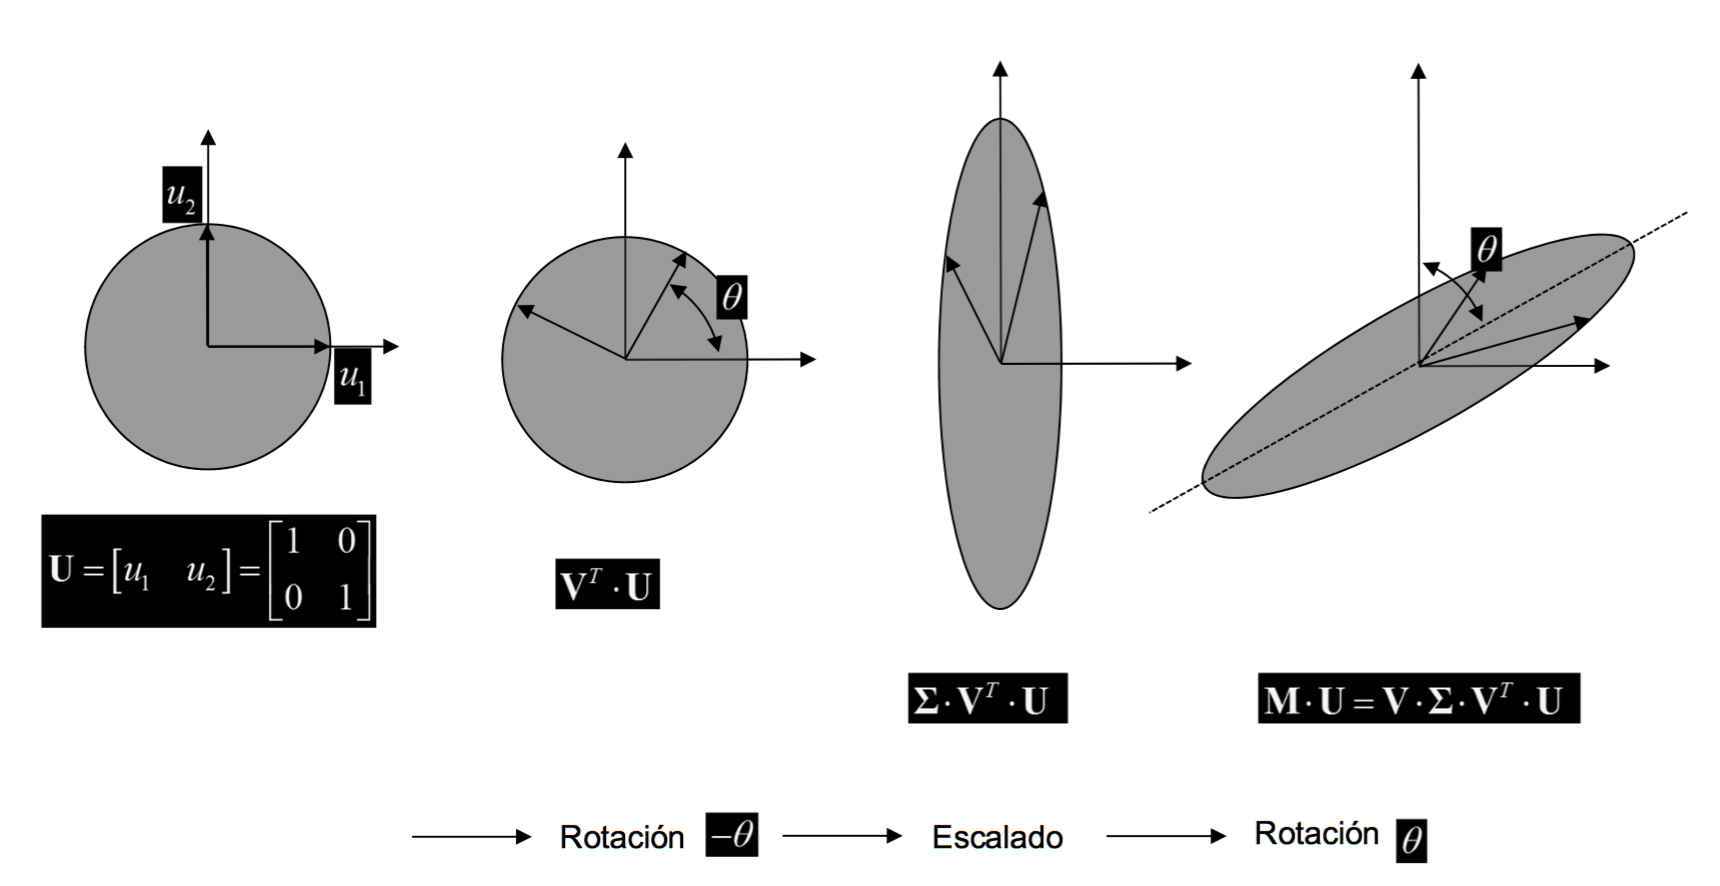
\includegraphics[width=0.8\textwidth]{img/Autovalores.png}
\caption{Interpretación geométrica de los autovalores viendo en qué transforman la bola unitaria.}
\label{fig:Autovalores}
\end{figure}

Los autovalores tienen una interpretación geométrica (ver \fref{fig:Autovalores}) que no se por qué podría resultar interesante pero que en cualquier caso es bastante obvia.

\subsection{Detección de puntos de interés}

La idea es buscar de forma precisa y robusta a ruido puntos invariantes a transformaciones típicas en la imagen. Hay varios métodos que pasamos a ver.

\subsubsection{Detector de Harris-Stephens}

Este detector se basa en un primer enfoque de fuerza bruta: cogemos una ventana en la imagen, la desplazamos un poquito y vemos en qué dirección cambia menos. Si no cambia en ninguna dirección, tenemos una zona plana. Si cambia muy poco en dos direcciones, tenemos un borde. Si cambia mucho en todas, probablemente estemos ante una esquina. Ese cambio se puede definir usando la suma de cuadrados de las diferencias.

Vamos a hacerlo algo formalmente. Tenemos nuestra imagen $\appl{ψ}{ℝ^2}{ℝ}$ y una ventana $W ⊂ ℝ^2$. Entonces, el error cuando desplazamos en la dirección del vector $\vu$ será \[ E(\vu) = \sum_{\vx ∈ W} \left(ψ(\vx + \vu) - ψ(\vx)\right)^2 \]

\begin{wrapfigure}{r}{0.4\textwidth}
\centering
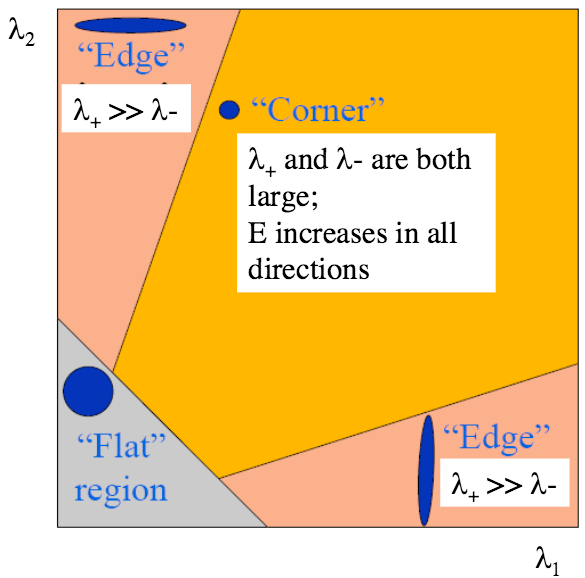
\includegraphics[width=0.32\textwidth]{img/StructureTensorEigenvalues.png}
\caption{Ilustración de los posibles casos según los autovalores de $A$}
\label{fig:StructureTensor}
\vspace{-10pt}
\end{wrapfigure}

Para desplazamientos pequeños, podremos aproximar la diferencia por el gradiente \[ ψ(\vx + \vu) \simeq ψ(\vx) + \vu · \grad ψ(\vx) \] de tal forma que nos queda \[ E(\vu) = \sum_{\vx ∈ W} \left(\vu \grad ψ(\vx)\right)^2 = \vu A \trans{\vu} \] con $A$ el tensor de estructura dado por \[ A =  \sum_{\vx ∈ W} \begin{pmatrix} ψ_x^2 (\vx) & ψ_x (\vx) · ψ_y (\vx) \\ ψ_x (\vx) · ψ_y (\vx) & ψ_y^2 (\vx) \end{pmatrix} \] (ojo: sólo primeras derivadas).

El estudio de autovalores y autovectores de $A$ nos dirá para dónde cambia la imagen y si tenemos un borde, esquina o región plana (\fref{fig:StructureTensor}). Sin embargo, como calcular los autovalores es computacionalmente caro, lo que se hace es hacer una estimación con la función de respuesta a una esquina, dada por \[ R(\vx) = λ_1λ_2 - κ (λ_1 + λ_2)^2 = \det A - κ \tr^2 A \] con $κ ∈ [0.04, 0.15]$ un parámetro que se ajusta experimentalmente.

Este enfoque es invariante a rotaciones y cambios de iluminación globales, pero tenemos el problema de la selección de κ y del umbral de $R$. Además, no es invariante a cambios de escala, y detecta más bien regiones que puntos de interés.

En la práctica, para calcularlo se sacan las imágenes de gradientes horizontales y verticales, se sacan las imágenes para la información del gradiente del tensor de estructura y por último se hace un filtrado gaussiano para obtener en cada píxel el tensor de estructura correspondiente de su entorno.

En otras palabras, lo que hace es estimar en el entorno de cada píxel la magnitud relativa del gradiente, en su dirección de máxima variación, con respecto a la que presenta en la dirección perpendicular.

Este detector se podría ampliar para localizar máximos/mínimos locales en el espacio escala que también sean máximos-minimos locales del laplaciano (Laplacian-Harris detector).

\subsubsection{SIFT - Scale-Invariant Feature Transform}

\begin{figure}[hbtp]
\centering
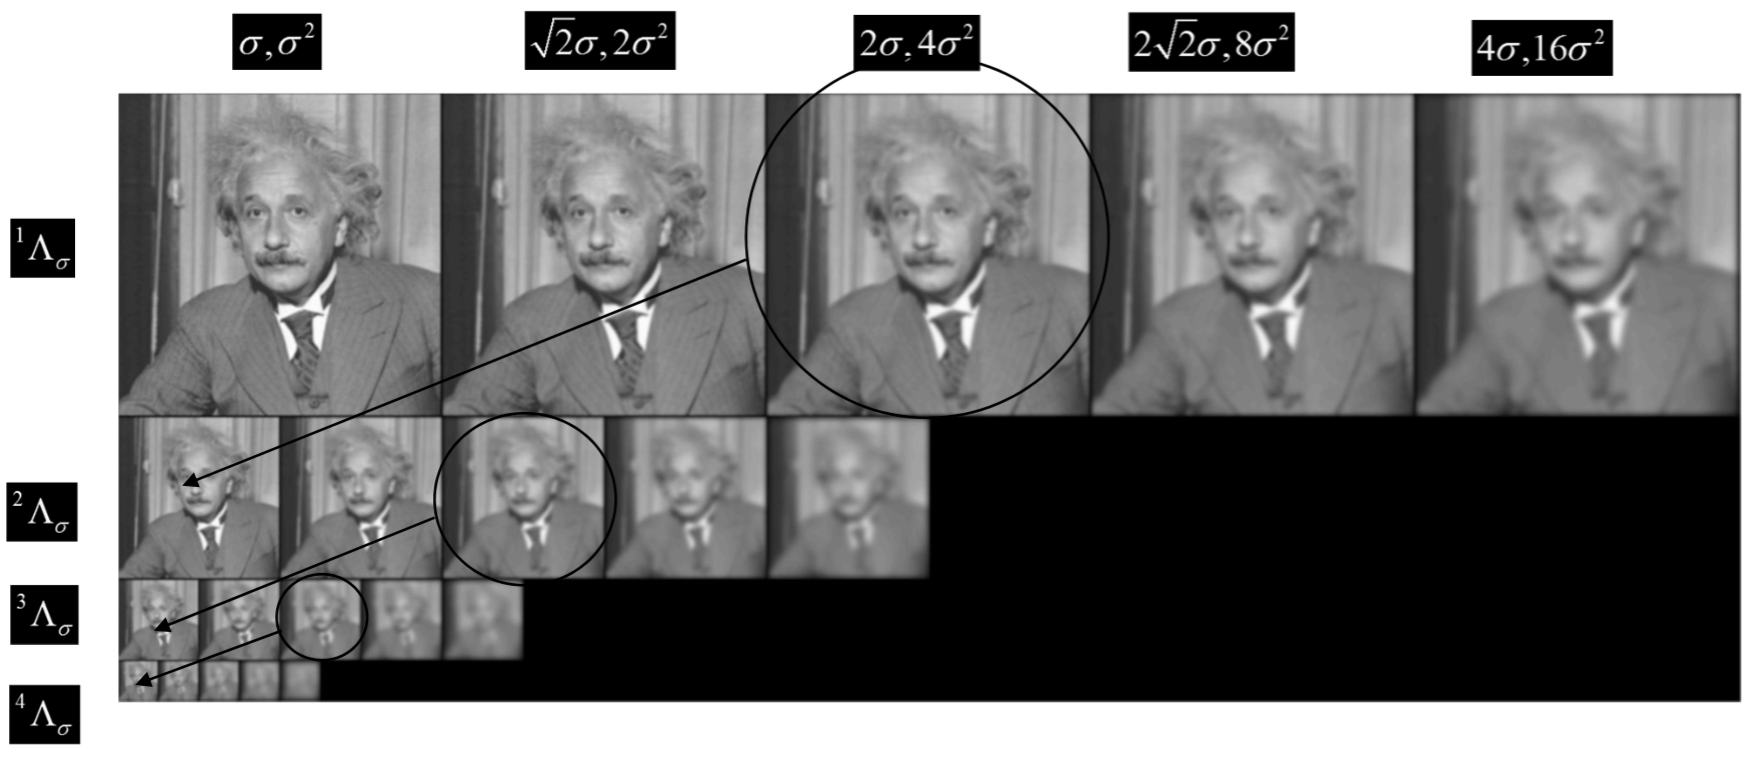
\includegraphics[width=0.8\textwidth]{img/SIFT.png}
\caption{Espacio escala híbrido: hacia la derecha suavizamos, hacia abajo diezmamos.}
\label{fig:SIFTScaleSpace}
\end{figure}

Este es un algoritmo avanzado para encontrar puntos de interés y describir su entorno. Es robusto a cambios de escala, traslaciones, rotaciones y cambios de iluminación; aunque no tanto a transformaciones afines y además tiene muchos parámetros a ajustar. Se basa en cuatro pasos: detección inicial de PoIs con la DoG en el espacio escala, localización precisa y descarte de PoIS, identificación de las orientaciones principales del gradiente y descripción del entorno en cada orientación principal.

El primer paso consiste en la obtención de un espacio escala híbrido (\fref{fig:SIFTScaleSpace}), obteniendo después las DoG en cada octava (entre cada suavizado), y se buscan máximos o mínimos locales en cada octava (de nuevo, comparando sólo con los vecinos de cada suavizado).

Una vez hecho esto, se refinan esos puntos de interés. Se mira qué desplazamiento $\vu$ minimiza (o maximiza) el valor de la DoG. Este valor vendrá dado por \[ \vu = - \left(\dpd[2]{D}{\vx}\right)^{-1} \pd{D}{\vx} \]. Si sus componentes son menores que $0.5$ se asume que el extremo está en la posición $\vx + \vu$. Si no, se asume que el extremo está más cerca del vecino correspondiente y se repite el proceso en torno a él.

Posteriormente se eliminan extremos poco contrastados, eliminando los que tengan $\abs{D(\vx)} ≤ 0.03$; y se quitan también los que forman arte de los bordes. Se calculan los Hessianos de esos puntos y se analiza la curvatura de la función $D(\vx)$. Si hay una curvatura con dirección predominante ($r = \sfrac{λ_1}{λ_2} > 10$) se descarta. Para facilitar este cálculo, se usa la traza y determinante del Hessiano y la desigualdad que se aplica es \[ \frac{\tr^2 HD(\vx)}{\det HD(\vx)} = \frac{(r + 1)^2}{r} > \frac{11^2}{10} \]

Sobre los puntos que quedan se computan unos descriptores basados en los ángulos del gradiente. Se coge una ventana de $16 × 16$ píxeles en la escala en la que aparece el punto, y se calcula el ángulo del gradiente en cada píxel. Se descartan los ángulos pequeños y entonces para cada subcelda de $4 × 4$ píxeles se calcula un histograma de las orientaciones que quedan rotadas con respecto a la orientación dominante (la que tenga el pico en el histograma), representadas como flechas de distinta magnitud en las ocho posibles direcciones que se puedan tomar. En la \fref{fig:SIFTDescritors} aparecen unos ejemplos del resultado de esos descriptores.

\begin{figure}[hbtp]
\centering
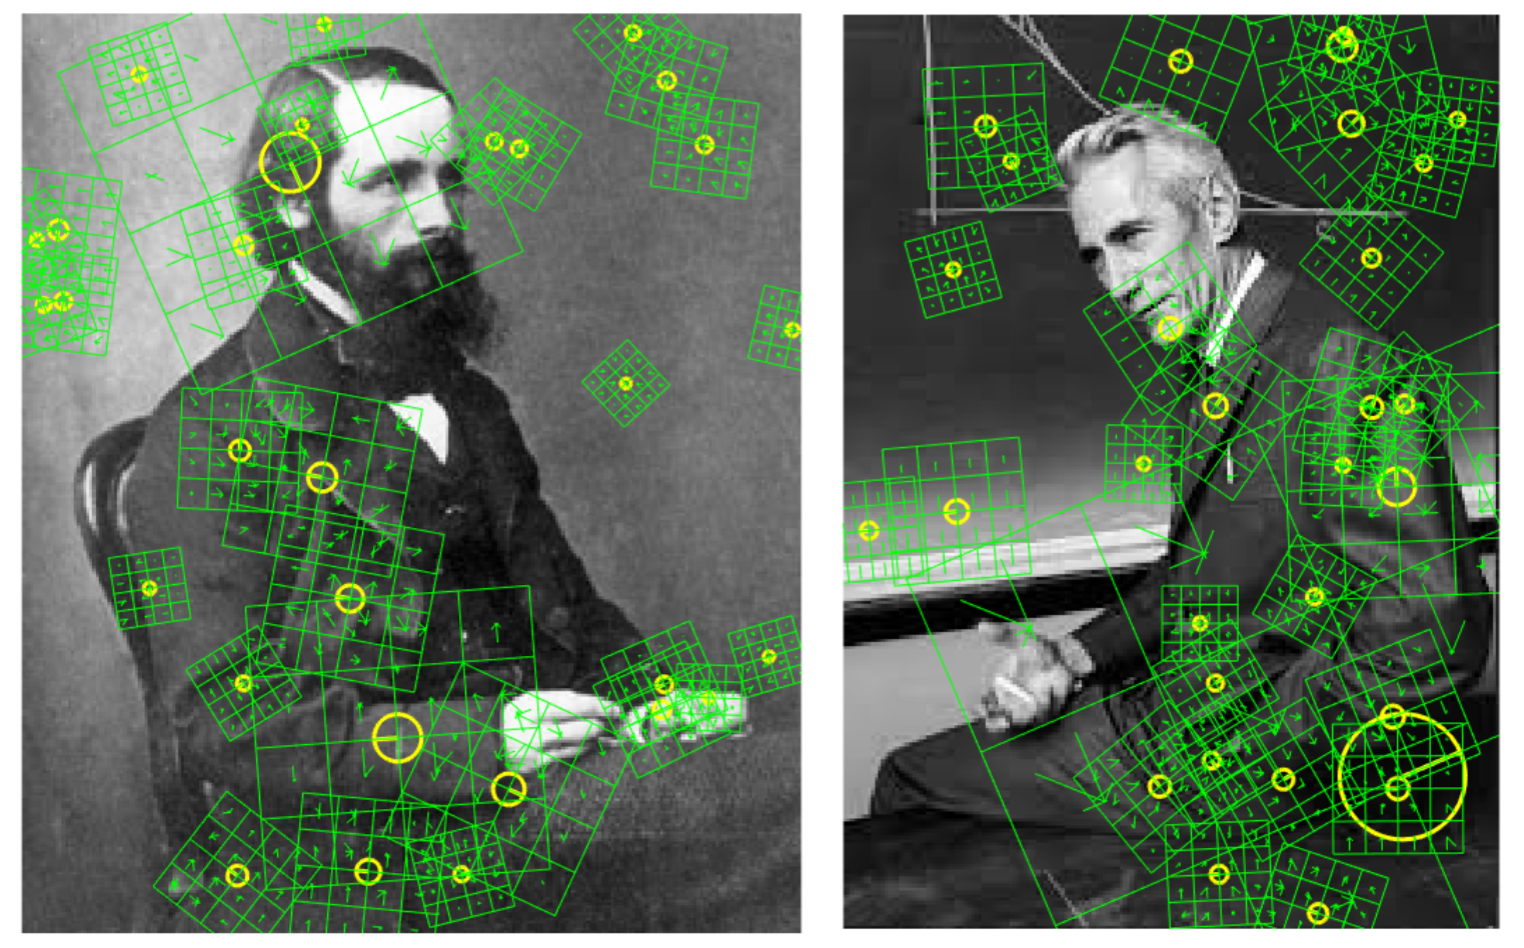
\includegraphics[width=0.8\textwidth]{img/SIFT_Descriptors.png}
\caption{Descriptores de SIFT sobre dos imágenes.}
\label{fig:SIFTDescritors}
\end{figure}

\subsubsection{SURF - Speeded Up Robust Features}

Se trata de un algoritmo rápido inspirado en SIFT de detección de puntos de interés y descripción de la región colindante. Se buscan los máximos del determinante del Hessiano de $L(\vx, σ)$ a cada escala. Para facilitar la computación, se aproximan las segundas derivadas de la gaussiana mediante filtros de caja (\fref{fig:FiltrosSURF}) cada vez más grandes y usando la imagen integral para mejorar el rendimiento. El detector devuelve regiones de interés (imagen de girasoles).

\begin{figure}[hbtp]
\centering
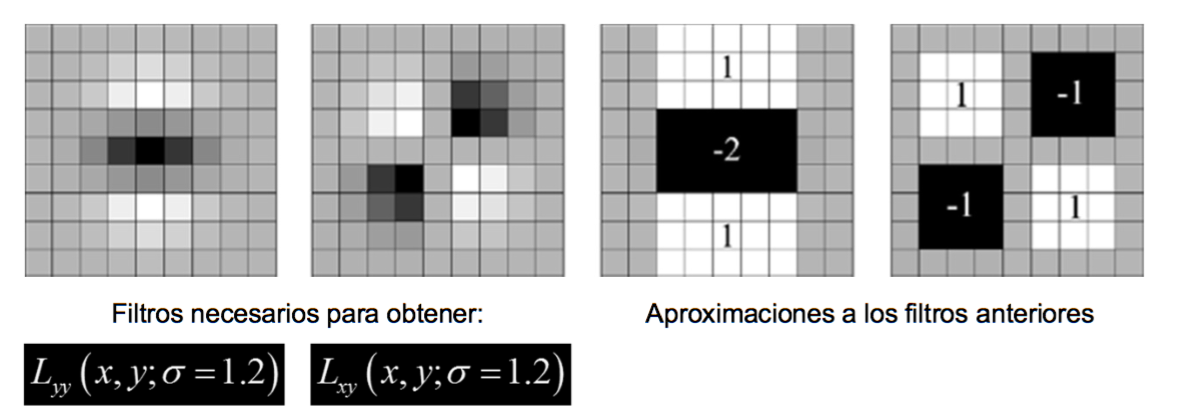
\includegraphics[width=0.8\textwidth]{img/FiltrosSURF.png}
\caption{Aproximación a la segunda derivada con filtros sencillos para SURF.}
\label{fig:FiltrosSURF}
\end{figure}

\subsubsection{MSER - Maximal Stable Extremal Regions}

Busca regiones asociadas a máximos o mínimos locales, y que son estables (variación mínima frente a cambios en el valor del umbral de luminancia).  Es robusta a variaciones del punto de vista, a cambio de escala y a cambios globales de iluminación, y es barato de computar.

A medida que se hace crecer el valor del umbral se obtienen las componentes conexas. Para cada componente se obtiene su área en función del umbral. Al final del proceso se buscan las regiones con un mínimo en el ritmo de cambio en el área, y con el umbral correspondiente se detecta la MSER.

\subsubsection{Descripción de regiones de interés}

Para describir las regiones de interés, hay dos algoritmos (aparte del de SIFT que ya hemos visto).

\paragraph{GLOH - Gradient Location and Orientation Histogram} Es prácticamente igual que el descriptor de SIFT, salvo porque la región entorno al punto de interés es circular, se divide en 17 regiones en forma log-polar, con el histograma de orientaciones cuantificado en 16 bins, lo que resulta en un vector descriptor de 17*16=272 componentes que luego se reduce aplicando PCA.

\paragraph{HOG - Histogram of Oriented Gradients}  Se describe una región rectangular (R-HOG) o circular (C-HOG) a partir de histogramas de orientación del gradiente de subregiones o celdas que pueden estar solapados. Es más bien un marco para adaptar a cada apliación. Para evitar variaciones de contraste, por ejemplo, se agrupan las celdas en bloques solapados. El vector concatena los histogramas de sus celdas.

\subsection{Detección y extracción de contornos}

\subsubsection{Algoritmo de Canny}

El principal algoritmo para esto es el algoritmo multietapa de Canny, que busca localizar todos los bordes de una imagen, con máxima precisión y sólo una vez cada borde. Su principal aportación es el cálculo de cruces por cero de la segunda derivada en la dirección del gradiente.

El algoritmo primero realiza un filtrado gaussiano y calcula el gradiente con los operadores de Prewitt o Sobel. Después, en cada entorno $3×3$ se analiza cada píxel (que contiene el valor del gradiente en ese punto): si el pixel central no es el máximo en la dirección del gradiente, entonces su magnitud se anula. Si la dirección del gradiente no es un divisible por $45$ grados, o bien se cuantifica en esos posibles valores o bien se interpola.

Luego se selecciónan dos umbrales: uno para identificar bordes muy marcados y otro algo menor para detectar bordes conectados con los anteriores. Asumiendo que los bordes pertenecen a contornos continuos, sobre la imagen de máximos del gradiente se seleccionan los píxeles mayores que el primer umbral y después se sigue en las direcciones perpendiculares al gradiente seleccionando píxeles conectados que superen el segundo umbral.

\subsubsection{Transformada de Hough}

El siguiente paso es la transformada de Hough, que basada en un esquema de votaciones permite localizar formas regulares básicas en imágenes binarias aunque no estén perfectamente definidas. El primer paso es pasar de la expresión en rectas a partir de los parámetros $m,b$ de la ecuación $y = mx + b$, que no están acotados, a otro espacio de parámetros $(r,θ)$ más cómodo (\fref{fig:RectasRTheta}). Así, cada punto $(x,y)$ de la imagen se transforma en una sinusoide del espacio $(r,θ)$, donde cada punto de esa sinusoide es una posible recta de la imagen binaria  que pasa por el punto $(x,y)$. El punto donde más sinusoides se crucen indican las rectas en la imagen.

\begin{figure}[hbtp]
\centering
\begin{tikzpicture}[scale=1.2]
\draw[->] (-0.1, 0) -- (5, 0) node [right] {$x$};
\draw[->] (0, -0.1) -- (0, 3) node [above] {$y$};

\coordinate (LBegin) at (0,2);
\coordinate (LEnd) at (4,0);
\coordinate (O) at (0,0);
\coordinate (I) at ($(LBegin)!(O)!(LEnd)$) {};
\coordinate (XEnd) at (3,0);

\draw[thick, blue] (LBegin) -- node[midway, above, anchor=south west] {$y = mx + b \equiv r = y\sin θ + x \cos θ$} (LEnd);
\draw[green!80!black] (I) -- node[midway, above, sloped] {$r$} (O);

\tikzangle[name={$\theta$}]{O}{I}{LEnd}

\end{tikzpicture}
\caption{Una recta se puede modelar con dos parámetros, $r$ y θ, sabiendo que $m = -\frac{\cos θ}{\sin θ}$ y que $b = \frac{r}{\sin θ}$.}
\label{fig:RectasRTheta}
\end{figure}

La ventaja de este proceso es que es robusto a ruido y a discontinuidades en los contornos. Eso sí, hay que buscar máximos en entornos para evitar tener haces de rectas.

\begin{wrapfigure}{r}{0.4\textwidth}
\centering
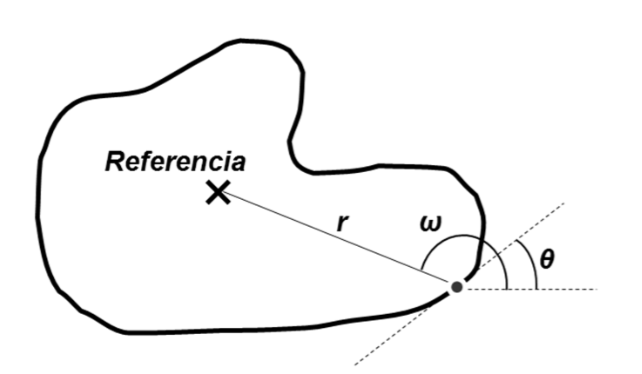
\includegraphics[width=0.4\textwidth]{img/HoughGeneral.png}
\caption{Esquema para asignar a cada $θ$ una serie de valores $(ω,r)$ en la transformada de Hough generalizada.}
\label{fig:HoughGeneral}
\end{wrapfigure}

La transformada de Hough también se puede aplicar a circunferencias: se hace un espacio de parámetros de tres dimensiones (centro $(a,b)$ y radio $r$) de la circunferencia. Igualmente, se puede generalizar a formas arbitrarias. Dada una forma de referencia con un centro, generamos una tabla R que a cada orientación $θ$ de la tangente le asigna varios puntos $(ω,r)$ con las coordenadas polares del punto del contorno (\fref{fig:HoughGeneral}).

A la hora de localizar las instancias de ese modelo, para cada píxel de un borde se estima la orientación de la recta tangente y para cada posible par $(ω,r)$ se incrementa el contador de la posición candidata del punto de referencia.

Este algoritmo también serviría para buscar la misma forma rotada por α, simplemente buscando las tuplas correspondientes al ángulo $θ-α$ e incrementando el contador la posición que tuviese radio $r$ y coordenadas $ω + α$. Igualmente, se puede hacer invariante a escalado poniendo como posición candidata la que tiene radio $rβ$.

\subsection{Seguimiento y aproximación de bordes}

Permite extraer y caracterizar las secuencias de píxeles de los diferentes segmentos de borde presentes en el resultado de un detector de bordes de grosor de un píxel, e identificar formas elementales, por ejemplo rectas. Consta de dos pasos que se van repitiendo en bucle: se selecciona el primer píxel que aparezca como borde al recorrer la imagen, y después se va siguiendo el borde usando codificación de Freeman (\fref{fig:Freeman}) para guardar la secuencia de bordes. Esos píxeles se suprimen, y se repiten los pasos hasta que no quedan mas píxeles en la imagen.

\begin{figure}[hbtp]
\centering
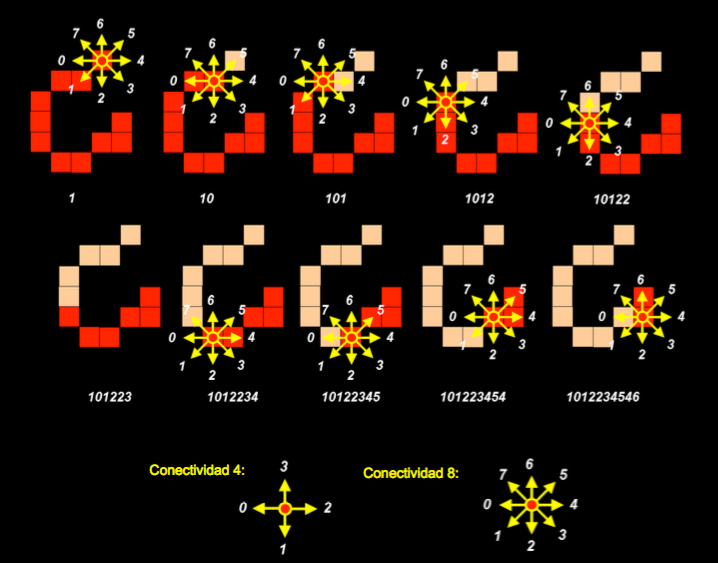
\includegraphics[width=0.8\textwidth]{img/Freeman.png}
\caption{Codificación Freeman para secuencia de píxeles}
\label{fig:Freeman}
\end{figure}

El seguimiento de contornos puede usarse para aproximar curvas por tramos rectos (obviamente). Esas secciones rectas pueden usarse como alternativa a la transformada de Hough.

\section{Introducción a la segmentación}

La segmentación busca definir conjuntos $Ω_j$ de píxeles similares conectados, homogéneos con respecto a alguna característica que representan una parte del espacio distinta al resto. Normalmente se asigna un identificador a cada región (etiqueta) y un representante, un descriptor de las características de la región.

El problema de la segmentación es que no está bien condicionada: depende de la escala, del conocimiento previo y de la relevancia que le demos a distintos detalles.

Las ventajas de la segmentación son ayudar a la descripción de imágenes y reducir la variablidad de los datos analizados, además de poder reducir ruido y de poder auto-definir la región de interés alrededor de un punto de interés.

La primera técnica es el clustering o agrupamiento por $k$-means o $c$-means, que busca particionar los puntos en $k$ subconjuntos para minimizar la distancia entre cada punto y la media de la región en la que está.

\begin{figure}[hbtp]
\centering
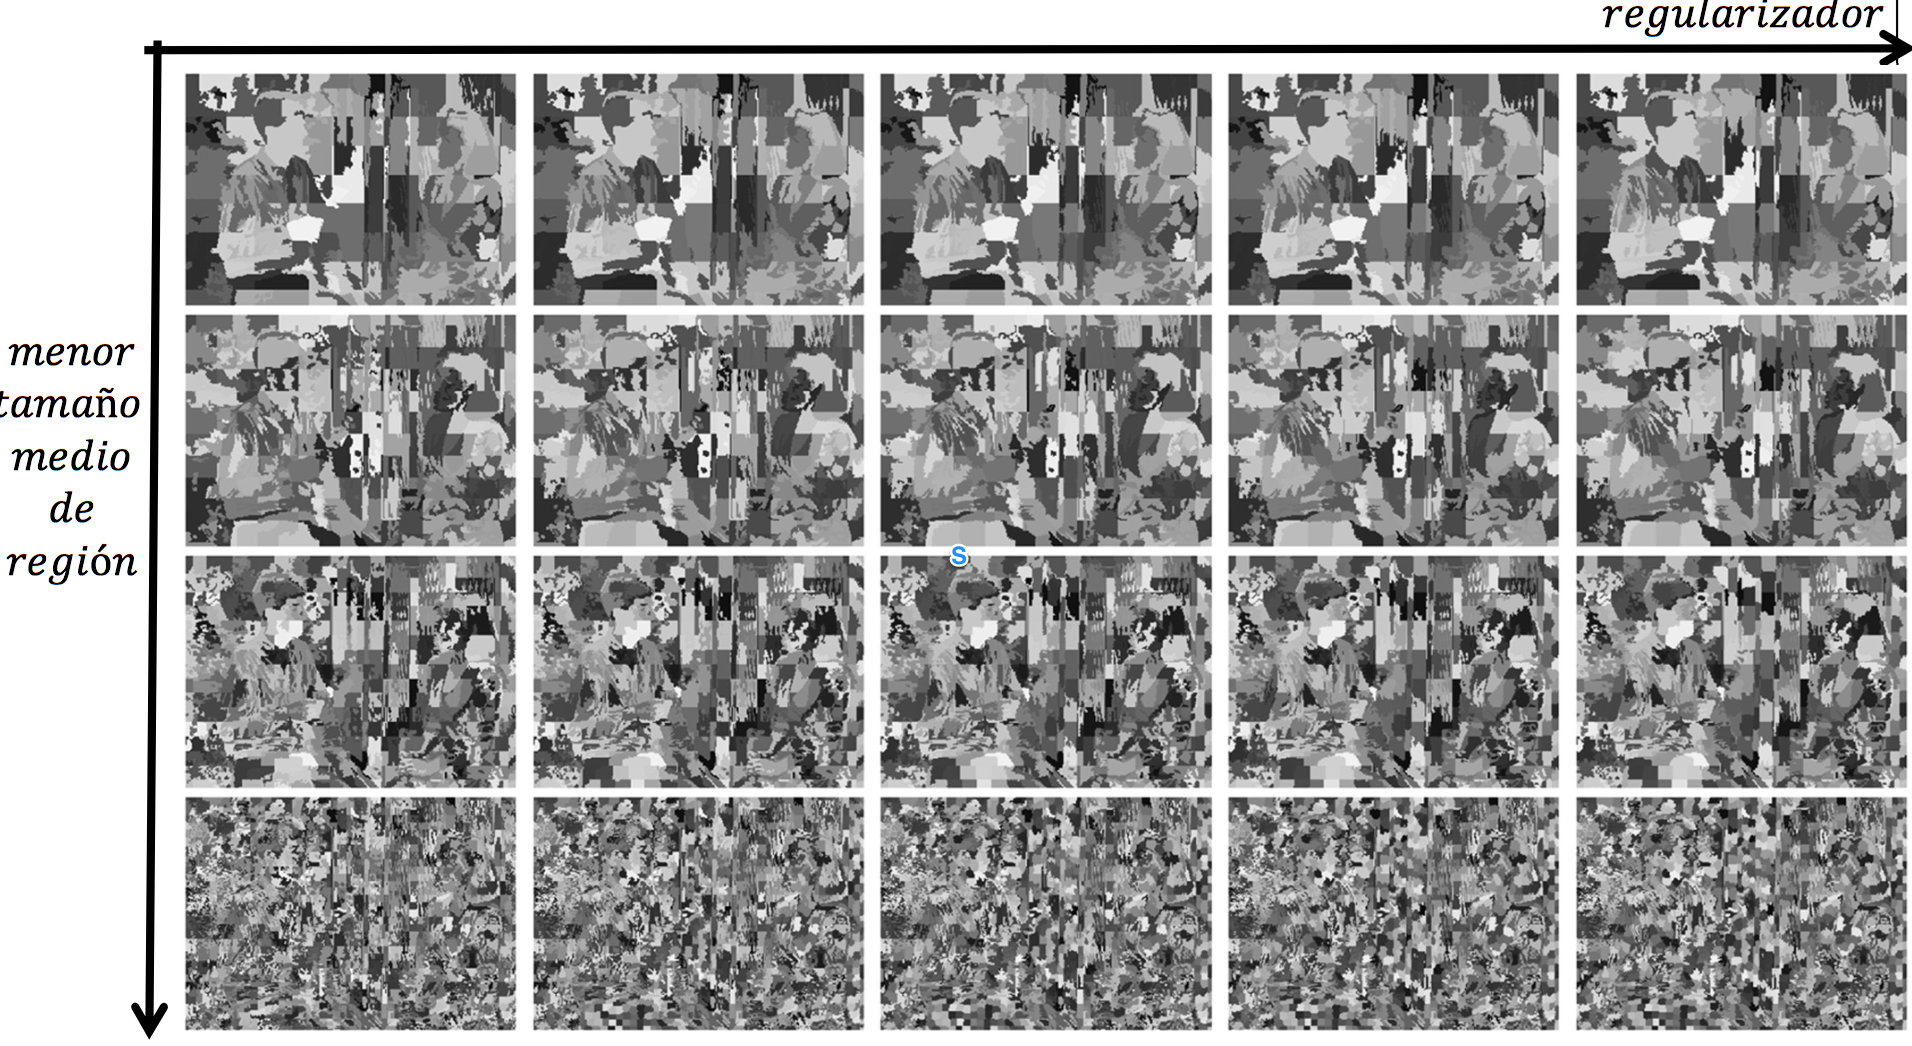
\includegraphics[width=0.8\textwidth]{img/Superpixels.png}
\caption{Efecto de los parámetros de la segmentación en superpíxeles.}
\label{fig:Superpixeles}
\end{figure}

También se usan los superpíxeles, donde se divide la imagen en bloques, se hace $k$-means en cada bloque y después se caracteriza cada píxel según una función $f$ (por ejemplo, la luminancia $L$) con el vector $\begin{pmatrix}λx & λy & f(x,y)\end{pmatrix}$, donde $λ$ es el cociente entre el regularizador y el tamaño medio de región. Un λ más alto da regiones más rectangulares, mientras que si es más bajo da regiones más ajustadas a los objetos (\fref{fig:Superpixeles}).

La segmentación en superpíxeles se suele usar como un paso previo a otros algoritmos más avanzados, para reducir su coste computacional. Por eso da una sobresegmentación, pero no elimina mucha información.

Otra técnica es el Mean-Shift, que busca modas en el espacio de decisión asumiendo que la relación moda - región es biunívoca. Se puede considerar como una técnica de ascenso de gradiente hasta llegar a un máximo. Para obtenerlo, se fija una ventana entorno a cada muestra y se obtiene la media de valores de la muestra en esa ventana. Después se desplaza la ventana para centrarla en la media obtenida, repitiendo el proceso hasta que la media converge.

Es un método muy eficaz, y además elimina la necesidad de establecer el número de regiones deseadas. Lo malo es que depende mucho del ancho de banda de los núcleos.

El método de \textit{snakes} (serpientes) trata de minimizar la energía de un contorno controlando la energía interna (aumenta con la deformación, evita el sobreajuste), la externa (ajuste a contornos) y la restrictiva (restricciones \textit{ad hoc} de diseño).

También hay métodos basados en grafos, como el SWA (\textit{Segmentation by Weighted Aggregation}), que fusiona píxeles o regiones similares en cada nivel de la jerarquía buscando minimizar la saliencia. El resultado es una jerarquía de regiones que además permite almacenar y manejar texturas. Cada región tiene un nivel óptimo en el que se obtiene su máxima saliencia.

También está el Global PB: se detectan contornos con diferentes hipótesis en su orientación, se genera un grafo de disimilutid y se estudian los contornos en las componentes principales que quedan codificadas en el grafo. Así en general no entiendo nada este algoritmo pero la idea es que parece generar pocas regiones.




\end{document}
